% *******************************************************************************
% * Copyright (c) 2007 by Elexis
% * All rights reserved. This document and the accompanying materials
% * are made available under the terms of the Eclipse Public License v1.0
% * which accompanies this distribution, and is available at
% * http://www.eclipse.org/legal/epl-v10.html
% *
% *  $Id: abrechnung.tex 2932 2007-07-29 06:21:06Z rgw_ch $
%
%*******************************************************************************
% !Mode:: "TeX:UTF-8" (encoding info for WinEdt)

\section{Abrechnungsbezogene Views}
\subsection{Konsultationen nach Datum}
\begin{wrapfigure}{l}{7cm}
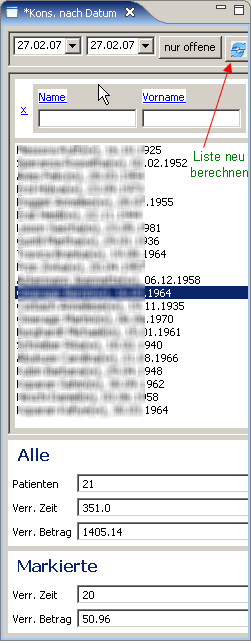
\includegraphics{images/konnd}
\caption{Konsultation nach Datum}
\label{fig:konnd}
\end{wrapfigure}
Diese View (s. Abb. \ref{fig:konnd}) dient dazu, Ihnen alle in einem bestimmten
Zeitraum stattgefundenen
Konsultationen aufzulisten. Sie können in den Datumsfeldern oben das Start- und
das Enddatum des gewünschten Zeitraums angeben.

Der Knopf \glqq nur offene\grqq kann betätigt werden, um in die Auflistung nur
solche Konsultationen aufzunehmen, für die noch keine Rechnung erstellt wurde.

Wenn Sie die Daten oder den Auswahlknopf geändert haben, erscheint die neu
berechnete Liste erst nach Klick auf den Button \glqq Liste neu berechnen\grqq.

Im unteren Abschnitt der View sehen Sie die Gesamtzahl der Konsultationen im
gewählten Zeitraum, sowie die (vom Abrechnungssystem her vorgegebene)
verrechnete Zeit und den verrechneten Betrag. Im Feld darunter sehen Sie
dieselben Angaben für die aktuell markierte Konsultation.

Sie können diese View also auch verwenden, um Abends kurz die Konsultationen des Tages
durchzugehen um unverrechnete oder falsch verrechnete zu korrigieren. Die Liste
kann auch zur einfacheren Lesbarkeit ausgedruckt werden (\textsc{ViewMenu-Liste drucken})

\clearpage

\subsection{Konsultationen zum Verrechnen}
\index{Abrechnung} Diese View (s. fig. \ref{fig:konsv}) dient dazu, diejenigen
Konsultationen
auszuwählen, von welchen eine Rechnung erstellt werden soll. Es werden dabei nur
die Konsultationen des aktuellen Mandanten angezeigt.
\begin{figure}[hb]
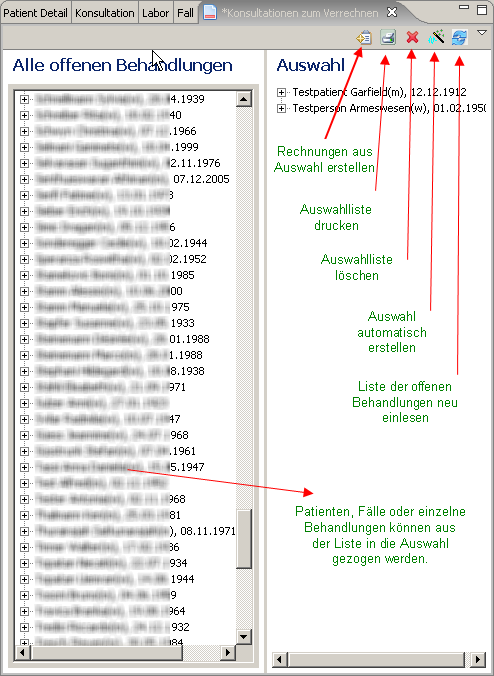
\includegraphics{images/konsv}
\caption{Konsultation zur Verrechnung auswählen}
\label {fig:konsv}
\end{figure}
Hierzu gibt es folgende Möglichkeiten:
\begin{itemize}
  \item Automatische Auswahl (Zauberstab-Icon): Dabei werden die Konsultationen nach bestimmten Regeln automatisch ausgewählt und in die Auswahlliste
  übertragen.
  \item Patientennamen aus der Liste in die Auswahl ziehen: Dadurch werden alle
  Konsultationen aller Fälle des gewählten Patienten zur Abrechnung markiert.
  \item Fälle aus der Liste in die Auswahl ziehen: Dadurch werden alle
  Konsultationen der gewählten Fälle zur Abrechnung markiert.
  \item Konsultationen aus der Liste in die Auswahl ziehen: Dadurch werden nur
  die gewählten Konsultationen zur Abrechnung vorgemerkt.
\end{itemize}
Bei allen Methoden können Sie die Auswahl nachträglich noch beliebig ändern. Sie
können weitere Elemente zufügen, oder Sie können (nach Rechtsklick auf ein
Element in der Auswahl) Elemente entfernen, oder Sie können die ganze Auswahl
wieder löschen. Zu diesem Zeitpunkt sind noch keinerlei Änderungen der Daten
erfolgt.

Wenn Sie die Auswahl fertig erstellt haben, können Sie auf \glqq Rechnungen
erstellen\grqq klicken, dann werden Rechnungen für alle in der Auswahl
befindlichen Elemente erstellt. Dabei werden immer alle Konsultationen, die zu
einem Fall gehören, zusammengefasst. Wenn von einem Patienten also mehrere Fälle
in der Auswahl sind, werden auch mehrere Rechnungen erstellt.

\clearpage 

\subsection{Rechnungen}
\begin{figure}[ht]
  % Requires \usepackage{graphicx}
  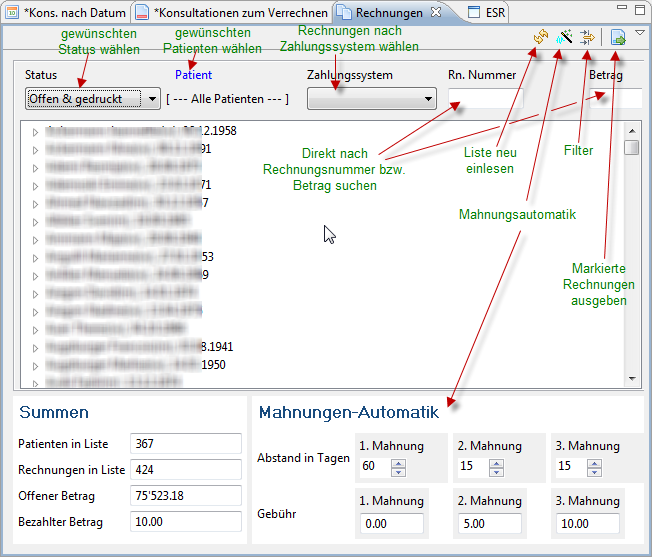
\includegraphics[width=0.8\textwidth]{images/rechnungsview}\\
  \caption{Rechnungen-View}\label{fig:rechnungen}
\end{figure}

In dieser View (Abb. \ref{fig:rechnungen}) sehen Sie die erstellten Rechnungen. Eine Rechnung hat immer einen bestimmten Status:
\begin{description}
    \item [Offen] Unmittelbar nach dem Erstellen.
    \item{Offen und gedruckt} Die Rechnung wurde mindestens einmal ausgegeben (über den Drucker oder eine andere Exportmethode). Ab diesem Zeitpunkt beginnt die Zahlungsfrist zu laufen. (Elexis kann allerdings nicht feststellen, ob beispielsweise der Drucker die Rechnung nicht korrekt ausgedruckt hat, oder ob sie nicht abgeschickt wurde. Deshalb liegt in diesem Punkt eine potentielle Fehlerquelle)
    \item[Zahlungserinnerung] Die Zahlungserinnerung wurde erstellt, aber noch nicht ausgedruckt
    \item[ZE gedruckt] Die Zahlungserinnerung wurdr ausgedruckt
    \item [2. Mahnung erstellt, 2. Mahnung gedruckt, 3. Mahnung erstellt, 3. Mahnung gedruckt]: analog
    \item[Teilweise bezahlt] Es ist (mindestens) eine Zahlung eingebucht, welche aber nicht den ganzen Rechnungsbetrag abdeckt.
    \item[bezahlt] Der Rechnungsbetrag wurde (in einer oder mehreren Buchungen) vollständig bezahlt
    \item [zuviel bezahlt] Auch das kommt vor.
    \item [Teilverlust] Ein Teil de Rechnungsbetrages wird abgeschrieben (Im Gegensatz zu \glqq Teilweise bezahlt\grqq{} rechnen Sie hier nicht mehr mit einer weiteren Zahlung)
    \item [Totalverlust] Der Rechnungsbetrag wird komplett abgeschrieben
    \item [In Betreibung] Genau das.
    \item [Storniert] Eine einmal erstellte Rechnung kann nicht mehr gelöscht werden. Das muss so sein, weil sonst die Situation möglich wäre, dass jemand eine nicht mehr existierende Rechnung reklamiert oder das Rückfragen zu einer inexistenten Rechnung kämen. Wenn eine Rechnung aus irgendeinem Grund ungültig ist (Fehler, Erlassen des Betrags etc.), dann muss sie stattdessen storniert werden. Stornieren hat in allen praktischen Belangen denselben Effekt wie löschen, ausser, dass die Rechnungsnummer vergeben bleibt und dass die Rechnung später wieder betrachtet werden kann.
    \item [fehlerhaft] Wenn ein Rechnungsausgabemodul feststellt, dass eine Rechnung fehlerhaft ist (beispielsweise könnte das TrustX-Modul monieren, dass nicht alle EAN-Nummern angegeben sind), dann erhält die betreffende Rechnung den Status fehlerhaft und kann so korrigiert werden.
    \item [zu drucken] Diese Einstellung findet alle Rechnungen, die offen, aber noch nicht gedruckt sind (also auch undegdurckte Mahnungen etc.)
\end{description}
Um die Rechnungen mit einem bestimmten Status anzuzeigen, wählen Sie diesen Status in der Combox links oben aus(S. Abb. \ref{fig:rechnungen}).
Um nur die Rechnungen eines betsimmten Patienten anzuzeigen, klicken Sie auf die bleuae Schrift \glqq Patient\grqq{}. Es öffnet sich die bekannte Kontaktauswahl-Dialogbox. Wählen Sie dort einen Patienten aus und klicken Sie ok, oder klicken Sie auf Abbrechen, um wieder alle Patienten anzuzeigen. Die Felder \glqq Datum von\grqq{} und \glqq Datum bis\grqq{} dienen dazu, nur Rechnungen auszuwählen, welche zwischen diesen Daten erstellt wurden. Wenn Sie auf die blaue Schrift Datum von oder Datum bis klicken, wechselt diese auf \glqq Status von\grqq{} bzw. \glqq Status bis\grqq{}. In diesem Fall werden diejenigen Rechnungen ausgewählt, bei denen die letzte \textit{Statusänderung} zwischen den angegebenen Daten liegt.
Das Feld \glqq Rn. Nummer\grqq{} ganz rechts dient schliessklich dazu, nur eine ganz bestimmte Rechnung mit dieser NUmmer herauszusuchen.

Wenn Sie die Felder wie gewünscht eingestellt haben, klicken Sie auf \glqq neu einlesen \grqq{}, dann wird die Liste anhand Ihrer Kriterien neu aufgebaut.
Unten sehen Sie jeweils die Zahl der mit diesen Kriterien vorhandenen Rechnungen, sowie die Summen.
\subsubsection{Rechnungen ändern}
Wenn Sie eine Rechnung der Liste mit der rechten Maustaste anklicken, können Sie diese Rechnung ändern:
\begin{itemize}
\item Ausgeben: Die Rechnung einzeln ausgeben (s. unten)
\item Buchung/Zahlung hinzufügen: Hier können Sie manuell Buchungen eingeben, z.B. wenn eine Barzahlung oder Anzahlung erfolgt ist. (Normalerweise erfolgen Buchungen via ESR automatisch).
\item Gebühr zuschlagen: Manuell z.B. Mahngebühr zufügen
\item Status ändern: Hier klann der Rechnungsstatus manuell geändert werden. Die meisten Statusänderungen erkennt Elexis automatisch. So werden z.B. beim Einlesen einer ESR-Datei von der Bank alle bezahlten Rechnungen automatisch auf \glqq bezahlt\grqq{} gesetzt etc. Manche Statusänderungen können aber nur manuell gemacht werden. Zum Beispiel kann Elexis den Unterschied zwischen \glqq Teilweise bezahlt\grqq{} und \glqq Teilverlust\grqq{} nicht automatisch erkennen, weil dies ja eine bewusste Entscheidung des Gläubigers ist. Dasselbe gilt für \glqq In Betreibung\grqq{} und \glqq Totalverlust\grqq{}.
    Von diesen Fällen abgesehen, sollten Sie aber vorsichtig sein mit manuellen Statusänderungen, da hierbei beispielsweise keine Buchungskorrekturen erfolgen.
\item Mahnstufe erhöhen: Hierdurch wird die Mahnstufe jeweils um eins erhöht bis max. Dritte Mahnung.
\item Stornieren: Damit wird die markierte Rechnung storniert. Man hat dabei die Möglichkeit, Behandlungen wieder freizugeben (z.B. wenn die Rechnung fehlerhaft war und neu erstellt werden soll), oder blockiert zu lassen (Wenn diese Behandlungen definitiv nicht verrechnet werden sollen).
\end{itemize}

\subsubsection{Rechnungen ausgeben}
Mit dem Button \glqq Rechnungen ausgeben\grqq{} werden alle markierten Rechnungen ausgegeben. (Um eine Rechnung zu markieren, klicken Sie mit der linken Maustaste auf diese. Um mehrere Rechnungen zu markieren, klicken Sie mit gedrückter Ctrl (bzw. Mac-) Taste auf die gewünschten Rechnungen. Um eine ganze Reihe zu markieren, klicken Sie zuerst auf die erste, dann mit gedrückter Shift-Taste auf die letzte Rechnung aus der Reihe.) Es wird also \textit{nicht} die ganze Liste ausgegeben, sondern nur die markierten Rechnungen!


Die möglichen Ziele der Rechnungsausgabe hängt von den installierten Abrechnungs-Plugins ab. Es kann zum Beispiel ein Drucker sein, der Tarmed-Rechnungen ausdruckt. Es kann aber auch eine XML-Datei oder direkt ein Trust-Center sein. Nähere Angaben dazu finden Sie in den entsprechenden Kapiteln (Tarmed: S. \pageref{arzttarife}, Trustx: S. \pageref{trustx})
\bigskip
Mit Klick auf das Zauberstab-Icon schliesslich setzen Sie die Mahnungen-Automatik in Gang. Diese wählt Rechnungen anhand der im unten rechts angezeigten Feld aus, erhöht die Mahnstufe, fügt wie gewünscht Gebühren zu und fasst diese Rechnungen als \glqq zu drucken\grqq{} zusammen.

\subsection{Konto}
\index{Konto}In dieser View sehen Sie alle Kontobewegungen eines bestimmten Patienten.
Rechnungen werden als negative, Zahlungen und Storno als positive
Buchungen erfasst, so dass Sie einfach über mehrere Rechnungen und Zahlungen
hinweg erkennen können, wo Sie finanziell mit dem betreffenden Klienten stehen.

\subsection{Konto-Liste}
Diese Liste zeigt alle Kontobewegungen insgesamt an.

\subsection{Leistungen}




